% =====================================================================
% AI Academy -- National AI Center -- MLE-AI-201 Machine Learning
% HW1 (Weeks 1-2) REPORT TEMPLATE
%
% This template imitates the IEEE two-column conference format WITHOUT
% depending on IEEEtran.cls or any special class file. It uses only the
% article class and packages that ship with every TeX distribution
% (geometry, graphicx, amsmath, amssymb). It compiles with pdflatex or
% tectonic out of the box.
%
% HOW TO USE:
%   1. Fill in the title block (your name + student ID).
%   2. Replace every [FILL IN ...] with your own content.
%   3. Put your plots in ../figures/ and include them with \includegraphics.
%   4. Compile:  pdflatex report_template.tex   (run twice for references)
%      or:       tectonic report_template.tex
%   5. Rename the output to report.pdf before submitting.
% =====================================================================

\documentclass[10pt,twocolumn,letterpaper]{article}

% ---- Minimal, always-available packages only -------------------------
\usepackage[T1]{fontenc}
\usepackage[utf8]{inputenc}
\usepackage[letterpaper,margin=0.75in,columnsep=0.25in]{geometry}
\usepackage{times}          % Times-like font, to mimic the IEEE look
\usepackage{amsmath,amssymb}
\usepackage{graphicx}
\usepackage{float}
\graphicspath{{figures/}{../figures/}}

% ---- Imitate the IEEE section styling by hand (no titlesec) ----------
\renewcommand{\thesection}{\Roman{section}}
\renewcommand{\thesubsection}{\Alph{subsection}}
\makeatletter
% Centered, small-caps section headings: "I. Introduction"
\renewcommand\section{\@startsection{section}{1}{\z@}%
  {3.5ex plus 1ex minus .2ex}{1.8ex plus .2ex}%
  {\centering\normalfont\normalsize\scshape}}
% Italic left-aligned subsection headings: "A. Subsection"
\renewcommand\subsection{\@startsection{subsection}{2}{\z@}%
  {3.0ex plus 1ex minus .2ex}{1.0ex plus .2ex}%
  {\normalfont\normalsize\itshape}}
\makeatother

% Tighter caption look, IEEE-ish
\renewcommand{\figurename}{Fig.}
\setlength{\parindent}{1em}

% =====================================================================
\begin{document}

% ---- TITLE BLOCK (spans both columns) -------------------------------
\twocolumn[
  \begin{center}
    {\LARGE\bfseries KNN, Metrics, and Regression from Scratch\par}
    \vspace{1.2em}
    {\large Alasgarov Teymur\par}
    \vspace{0.3em}
    {\normalsize Student ID: 3032 \quad\textbullet\quad Date: 30.09.2026\par}
    \vspace{0.3em}
    {\itshape MLE-AI-201 Machine Learning, Cohort II\\ AI Academy, National AI Center\par}
    \vspace{1.4em}
  \end{center}
]

% ---- ABSTRACT (IEEE style: bold-italic "Abstract" em-dash) ----------
\noindent\textbf{\textit{Abstract}}---\textit{%
In this report, I implemented KNN, four classification metrics (accuracy, precision, recall, and $\text{F}_1$), and batch gradient descent for both linear and logistic regression using only NumPy. For the Breast Cancer Wisconsin dataset, the KNN model achieved its best test $\text{F}_1$ score of 0.9727 at $k = 7$, with the results matching scikit-learn across all tested $k$ values. On the Diabetes dataset, the linear regression model achieved a test $R^2$ of 0.4774 ($\text{MSE} \approx 2821.28$), which was almost identical to scikit-learn's $R^2$ of 0.4773. The logistic regression model reached 0.9766 test accuracy and 0.9813 $\text{F}_1$ on the Breast Cancer dataset. Overall, the from-scratch implementations closely matched scikit-learn on KNN and linear regression, while logistic regression matched well on test metrics despite some divergence in the underlying learned weights.
}

\vspace{0.6em}
\noindent\textbf{\textit{Index Terms}}---\textit{k-nearest neighbors,
classification metrics, linear regression, logistic regression,
gradient descent, regularization.}

\vspace{0.8em}

% =====================================================================
\section{Introduction}
The main goal of this assignment is to understand how basic machine learning algorithms work by implementing them from scratch using only NumPy. This report covers KNN, common classification metrics, and batch gradient descent for linear and logistic regression, along with an optional comparison of L1 and L2 regularization. Each algorithm is tested on benchmark datasets and compared with scikit-learn to check that the implementations produce accurate and consistent results.

% =====================================================================
\section{KNN and Metrics}
\subsection{KNN implementation}
I implemented $k$-nearest neighbors without any Python loops over training points by vectorizing the pairwise Euclidean distance computation. Expanding the squared Euclidean distance as
\begin{equation}
  \lVert \mathbf{x}-\mathbf{z}\rVert_2^2
  = \lVert \mathbf{x}\rVert_2^2 - 2\,\mathbf{x}^\top\mathbf{z}
  + \lVert \mathbf{z}\rVert_2^2
\end{equation}
allows computing the full distance matrix $\mathbf{D} \in \mathbb{R}^{N_\text{test} \times N_\text{train}}$ in one operation using matrix multiplication ($\mathbf{X}_\text{test}\mathbf{X}_\text{train}^\top$) and NumPy broadcasting with the row squared norms. Nearest neighbor indices are retrieved via \texttt{np.argpartition}, and majority class voting is evaluated using \texttt{np.bincount}.

\subsection{Metrics implementation}
The classification metrics were implemented directly from the confusion matrix counts ($\text{TP}$, $\text{FP}$, $\text{TN}$, $\text{FN}$). Accuracy is computed as $(\text{TP}+\text{TN})/N$, precision as $\text{TP}/(\text{TP}+\text{FP})$, recall as $\text{TP}/(\text{TP}+\text{FN})$, and $\text{F}_1$ as the harmonic mean $2(\text{precision}\cdot\text{recall})/(\text{precision}+\text{recall})$. If any denominator was zero, the corresponding metric was set to (0.0) to avoid division-by-zero errors.

\subsection{Results}
We tested the KNN model with \(k \in \{1, 3, 5, 7, 9, 11, 15, 21\}\) using standardized features from the Breast Cancer dataset (Fig.~\ref{fig:knn}). The best \(F_1\) score was \(0.9727\) at \(k=7\), although the same score was also achieved with \(k=9\) and \(k=11\). At these values, the model had a precision of \(0.9469\) and a recall of \(1.0000\). As shown in Table~\ref{tab:knn}, the from-scratch implementation produced exactly the same predictions and metric values as scikit-learn for every tested \(k\).

% ---- Example table (plain tabular, no booktabs dependency) ----------
\begin{table}[ht]
  \centering
  \caption{Test-set metrics for the best $k=7$ (breast cancer).}
  \label{tab:knn}
  \begin{tabular}{lcccc}
    \hline
    Model & Acc & Prec & Rec & F$_1$ \\
    \hline
    Custom KNN ($k{=}7$) & 0.9649 & 0.9469 & 1.0000 & 0.9727 \\
    sklearn KNN ($k{=}7$) & 0.9649 & 0.9469 & 1.0000 & 0.9727 \\
    \hline
  \end{tabular}
\end{table}

% ---- Example figure -------------------------------------------------
\begin{figure}[ht]
  \centering
  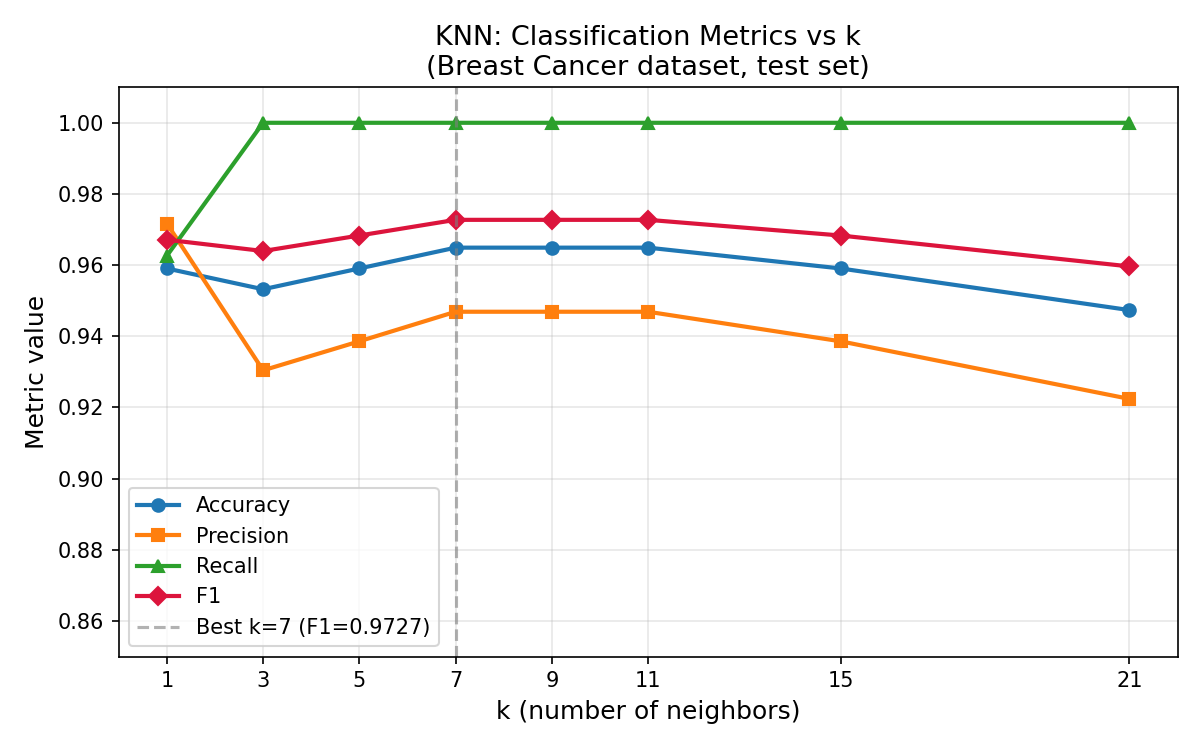
\includegraphics[width=\linewidth]{knn_metrics_vs_k.png}
  \caption{Test-set classification metrics across different values of $k$ on the Breast Cancer dataset.}
  \label{fig:knn}
\end{figure}

% =====================================================================
\section{Linear and Logistic Regression}
\subsection{Linear regression}
Linear regression was implemented using batch gradient descent on the mean-squared-error (MSE) loss function. With standardized features on the Diabetes dataset, a learning rate $\eta = 0.1$, and $1000$ epochs, parameters were updated iteratively as $\mathbf{w} \leftarrow \mathbf{w} - \eta \nabla_{\mathbf{w}}J$ and $b \leftarrow b - \eta \nabla_b J$.

The mean-squared-error objective and its gradient are
\begin{equation}
  J(\mathbf{w},b) = \frac{1}{N}\lVert \mathbf{X}\mathbf{w}+b-\mathbf{y}\rVert_2^2,
  \quad
  \nabla_{\mathbf{w}}J = \frac{2}{N}\mathbf{X}^\top(\mathbf{X}\mathbf{w}+b-\mathbf{y}).
\end{equation}
On the 30\% test set, the model achieved an MSE of $2821.28$ and an $R^2$ of $0.4774$, which was very close to scikit-learn's results of MSE $= 2821.75$ and $R^2 = 0.4773$. The small difference comes from gradient descent approaching the solution iteratively, while scikit-learn uses a closed-form solution based on SVD.

\subsection{Logistic Regression}

Logistic regression was implemented from scratch using batch gradient descent with binary cross-entropy loss on the Breast Cancer dataset. The model calculated predicted probabilities using a numerically stable sigmoid function, with a learning rate of $\eta = 0.1$ and $1000$ training epochs.

The sigmoid function and gradient used for the updates are

\begin{equation}
    \sigma(z)=\frac{1}{1+e^{-z}},
    \quad
    \nabla_{\mathbf{w}}J=\frac{1}{N}\mathbf{X}^\top(\hat{\mathbf{p}}-\mathbf{y}).
\end{equation}

On the test set, the model achieved an accuracy of $0.9766$, precision of $0.9813$, recall of $0.9813$, and an $\text{F}_1$ score of $0.9813$. These results were close to the scikit-learn unregularized L-BFGS baseline, which achieved an accuracy of $0.9649$ and an $\text{F}_1$ score of $0.9725$. The small difference is mainly due to the standardized Breast Cancer data being close to separable, so different optimization methods and stopping criteria can converge to slightly different solutions.

\subsection{Training curves}
Fig.~\ref{fig:linear_loss} and Fig.~\ref{fig:logistic_loss} show the training loss curves over $1000$ epochs for linear and logistic regression. In both cases, the loss decreases monotonically and flattens out smoothly, confirming that the learning rate $\eta = 0.1$ is well-suited and ensures stable convergence.

\begin{figure}[H]
  \centering
  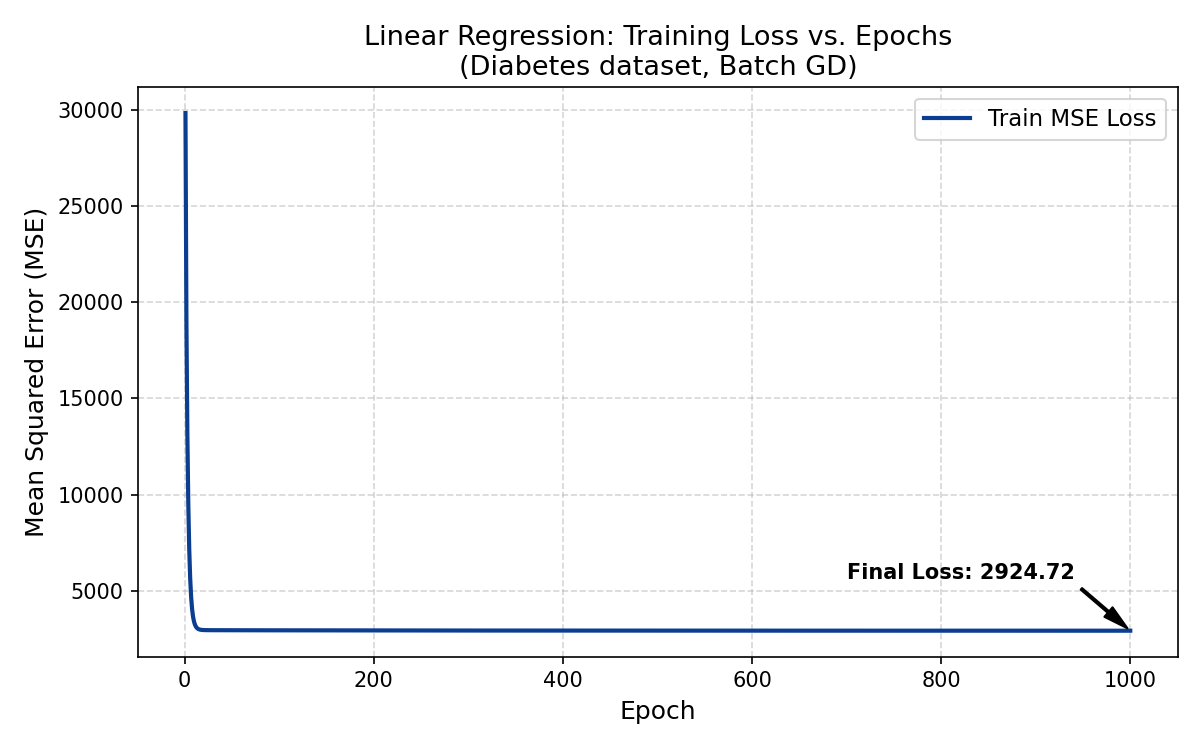
\includegraphics[width=0.74\linewidth]{linear_loss.png}
  \caption{MSE loss vs.\ epoch during Linear Regression gradient descent.}
  \label{fig:linear_loss}
\end{figure}

\begin{figure}[H]
  \centering
  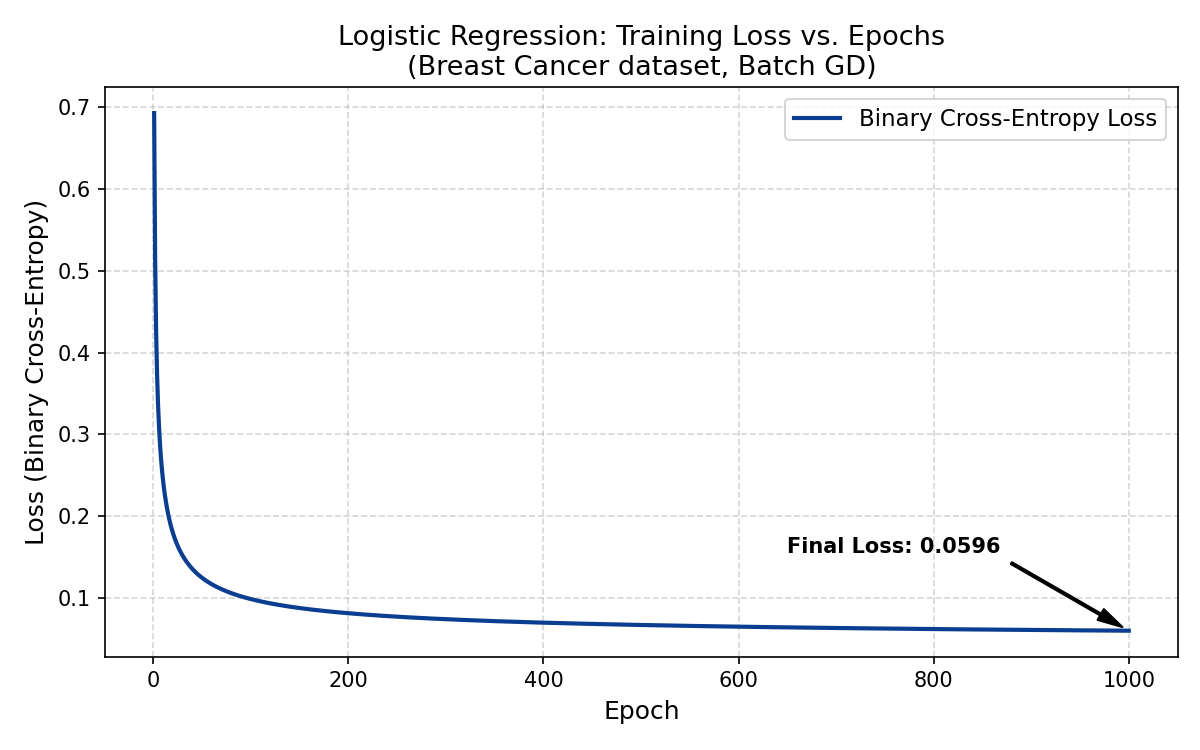
\includegraphics[width=0.74\linewidth]{logistic_loss.png}
  \caption{Binary cross-entropy loss vs.\ epoch during Logistic Regression.}
  \label{fig:logistic_loss}
\end{figure}

% =====================================================================
\section{Bonus: Regularization (optional)}
I implemented both \(L_1\) regularization (Lasso using subgradient descent) and \(L_2\) regularization (Ridge using weight decay) for Linear Regression on the Diabetes dataset, testing \(\lambda \in \{0, 0.001, 0.01, 0.1, 1.0, 5.0\}\). 

With \(L_1\) regularization, increasing \(\lambda\) pushed some feature weights closer to zero and made the model sparser (Fig.~\ref{fig:reg_l1}). For example, at \(\lambda=1.0\), Feature 5 decreased to \(w_5 \approx 0.076\), while the overall \(||w||_1\) decreased from 163.13 to 106.20. With \(L_2\), the weights decreased more smoothly without becoming exactly zero (Fig.~\ref{fig:reg_l2}), with \(||w||_2\) falling from 63.32 at \(\lambda=0\) to 11.43 at \(\lambda=5.0\). Small amounts of regularization (\(\lambda \le 0.1\)) kept the test \(R^2\) around 0.48, while stronger regularization, such as \(L_2\) with \(\lambda=5.0\), reduced the test \(R^2\) to 0.2852, indicating over-penalization.

\begin{figure}[H]
  \centering
  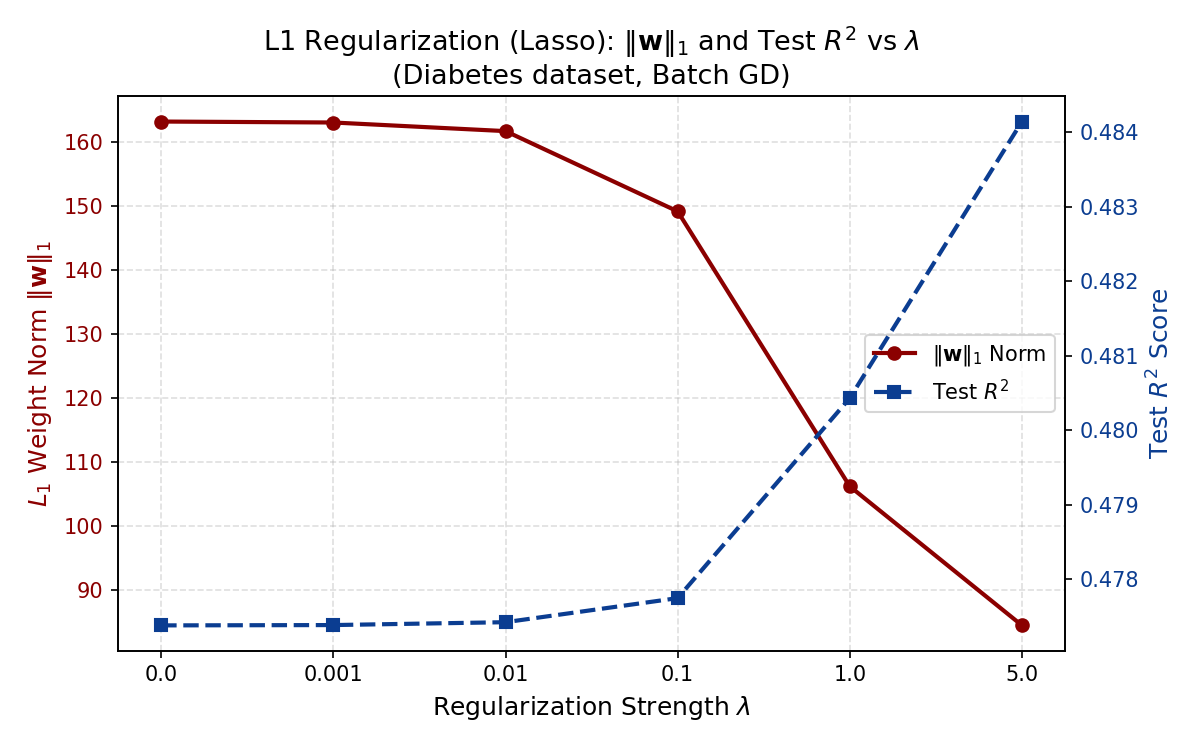
\includegraphics[width=0.74\linewidth]{reg_l1.png}
  \caption{$L_1$ weight norm and test performance vs.\ $\lambda$.}
  \label{fig:reg_l1}
\end{figure}

\begin{figure}[H]
  \centering
  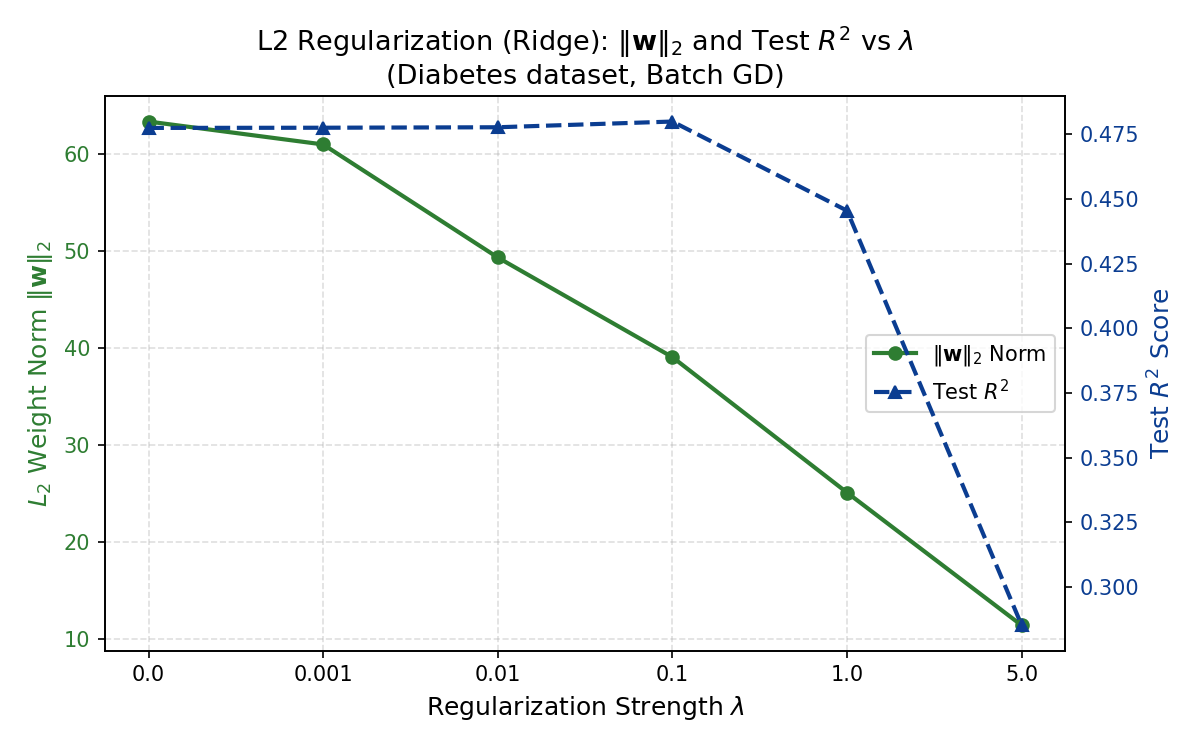
\includegraphics[width=0.74\linewidth]{reg_l2.png}
  \caption{$L_2$ weight norm and test performance vs.\ $\lambda$.}
  \label{fig:reg_l2}
\end{figure}

% =====================================================================
\section{Conclusion}
The from-scratch implementations worked well and produced results very close to scikit-learn. I was surprised by how small the differences were, especially for KNN and the classification metrics. The small differences in linear regression mainly came from gradient descent reaching the solution step by step instead of calculating it directly with the closed-form method. For logistic regression, the differences were mostly caused by the standardized Breast Cancer data being almost perfectly separable, so the unregularized model does not have a finite minimum. As a result, different optimization methods and stopping criteria can end up at slightly different points during training.

% =====================================================================
\section*{AI-Tool Usage Declaration}
An LLM assistant was consulted during this assignment to look up NumPy broadcasting syntax (specifically for vectorized Euclidean distance computation), Matplotlib plotting/styling templates for generating figures, and LaTeX formatting/syntax commands.

% =====================================================================
\begin{thebibliography}{9}
\bibitem{islp} G.~James, D.~Witten, T.~Hastie, R.~Tibshirani, and J.~Taylor,
  \textit{An Introduction to Statistical Learning with Applications in Python}. Springer, 2023.
\bibitem{esl} T.~Hastie, R.~Tibshirani, and J.~Friedman,
  \textit{The Elements of Statistical Learning}, 2nd ed. Springer, 2009.
\bibitem{sklearn} F.~Pedregosa et al., ``Scikit-learn: Machine learning in Python,''
  \textit{JMLR}, vol.~12, pp.~2825--2830, 2011.
\end{thebibliography}

\end{document}
